\tikzset{
    arg/.style={
        draw,
        circle,
        fill=gray!15,
        inner sep=1pt,
        minimum size=.5cm
    }
}

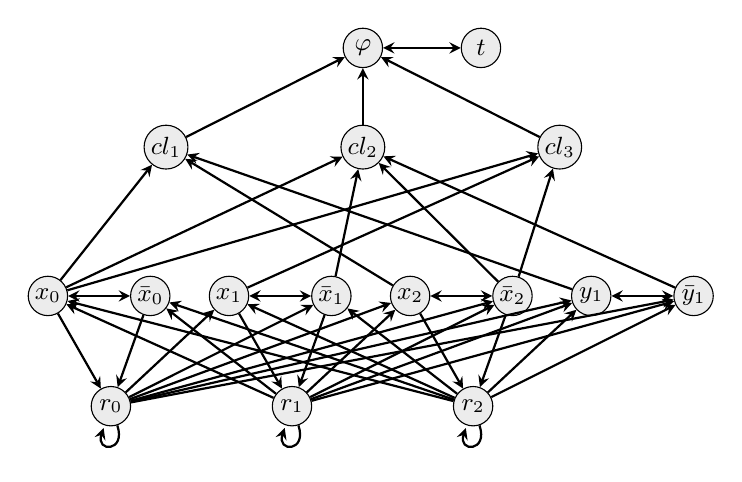
\begin{tikzpicture}[>=stealth,xscale=1, yscale=0.7]
\small
		\path
			node[arg] at (0,0.5) (phi) {$\varphi$}
			node[arg] at (1.5,0.5) (t) {$t$}
			;
		\path 	(-2.5,-1.3) 
			node[arg](c1){$cl_1$}
			++(2.5,0) node[arg](c2){$cl_2$}
			++(2.5,0) node[arg](c3){$cl_3$};
		\path 	(-4,-4) 
					node[arg](z1){$x_0$}
			++(1.3,0) node[arg](nz1){$\bar x_0$}
			++(1,0) node[arg](z4){$x_1$}
			++(1.3,0) node[arg](nz4){$\bar x_1$}
			++(1,0) node[arg](z2){$x_2$}
			++(1.3,0) node[arg](nz2){$\bar x_2$}
			++(1,0) node[arg](z3){$y_1$}
			++(1.3,0) node[arg](nz3){$\bar y_1$}
			;
        \path 	(-3.2,-6) 
					node[arg](r1){$r_0$}
			++(2.3,0) node[arg](r2){$r_1$}
			++(2.3,0) node[arg](r3){$r_2$}
            ;
		  \path [->,thick,loop below]
			(r3) edge (r3)
			(r2) edge (r2)
			(r1) edge (r1)
			;  
        \path [->, thick]
			(z4) edge (r2)
            (nz4) edge (r2)
			(z2) edge (r3)
            (nz2) edge (r3)
			(z1) edge (r1)
            (nz1) edge (r1)
			;     
			 
        \path [->,thick]
			(r3) edge (z1)
                 edge (z4)
                 edge (z3)
                 edge (nz3)
                 edge (nz1)
                 edge (nz4)
			(r2) edge (z1)
                 edge (z2)
                 edge (z3)
                 edge (nz3)
                 edge (nz1)
                 edge (nz2)
			(r1) edge (z2)
                 edge (z4)
                 edge (z3)
                 edge (nz3)
                 edge (nz2)
                 edge (nz4)
			;      
			
		\path [->,thick]
			(c3) edge (phi)
			(c2) edge (phi)
			(c1) edge (phi)
			;
			
		\path [left,->, thick]
			(z1) edge (c1)
			% (z1) edge[in=90,out=90] (c1)
			(z1) edge (c2)
			(z1) edge (c3)
			(z2) edge (c1)
			(z3) edge (c1)
			(nz2) edge (c2)
			(nz3) edge (c2)
			(nz4) edge (c2)
			(nz2) edge (c3)
			(z4) edge (c3)
			;
			
		\path [left,<->, thick]
			(z1) edge (nz1)
			(z2) edge (nz2)
			(z3) edge (nz3)
			(z4) edge (nz4)
            (phi) edge (t);
\end{tikzpicture}